\begin{figure}[p]
\centering
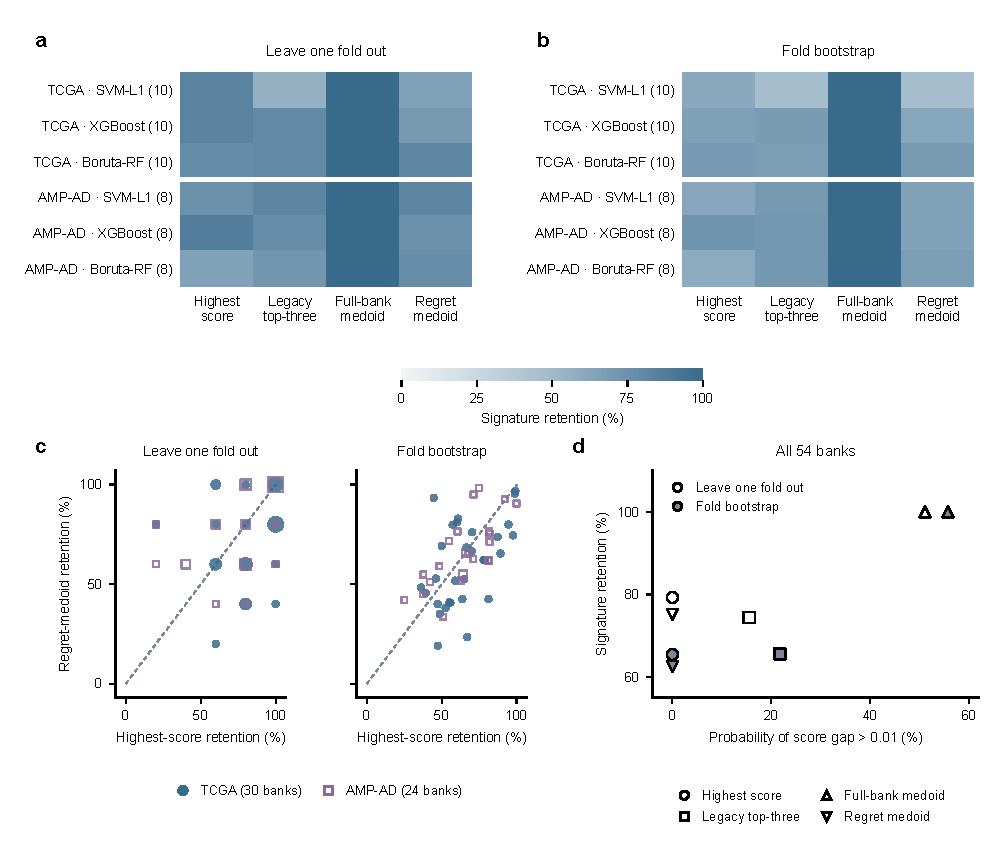
\includegraphics[width=170mm]{v19_work/supplement_polish_20261105/modern/figures/supp_figure_s29_cv_score_sensitivity.pdf}
\caption{Fixed-bank sensitivity to paired development-fold weighting in 54 five-candidate banks (30 TCGA, 24 AMP-AD). Masks and score arrays are fixed; candidates and rules share weights. Retention denotes recovery of each rule's uniform-weight mask. Leave-one-fold-out averages five omissions equally; bootstrap weighting uses multinomial probabilities for 126 count vectors (3,125 ordered resamples).
a,b) Equal-bank mean retention by cohort and branch; parentheses give bank counts.
c) Regret-medoid versus highest-score retention. The diagonal denotes equality; marker area counts exactly coincident banks within each cohort. Both facets reuse the same banks.
d) Equal-bank retention and probability that the perturbed bank-best-minus-selected score exceeds $\delta=0.01$. Open/filled symbols denote leave-one-fold-out/bootstrap weighting; shape denotes rule. Highest-score and regret-constrained exceedance is zero by definition. Unrestricted-medoid retention is 100\% because geometric winners are unchanged. Bootstrap exceedance is 55.76\% for unrestricted and 21.76\% for legacy top-three medoids; regret-medoid and highest-score retention is 62.55\% and 65.44\%, respectively.
Dependent fold scores are reweighted without refitting, held-out access, or participant/bank regeneration. These are descriptive sensitivities, not generalization intervals; no $p$ values are estimated. Mean gaps appear in Supplementary Table~S29.}
\label{fig:supp29}
\end{figure}
